\documentclass[10pt,twocolumn]{article}

% use the oxycomps style file
\usepackage{oxycomps}
\usepackage{listings}
\usepackage{xcolor}
\usepackage{geometry}
\usepackage{graphicx}
\usepackage{caption}

% Define custom colors for code listings
\definecolor{codegreen}{rgb}{0,0.6,0}
\definecolor{codegray}{rgb}{0.5,0.5,0.5}
\definecolor{codepurple}{rgb}{0.58,0,0.82}
\definecolor{backcolour}{rgb}{0.95,0.95,0.92}

% Define code listing style
\lstdefinestyle{mystyle}{
    backgroundcolor=\color{backcolour},
    commentstyle=\color{codegreen},
    keywordstyle=\color{magenta},
    numberstyle=\tiny\color{codegray},
    stringstyle=\color{codepurple},
    basicstyle=\footnotesize\ttfamily,
    breakatwhitespace=false,
    breaklines=true,
    captionpos=b,
    keepspaces=true,
    numbers=left,
    numbersep=5pt,
    showspaces=false,
    showstringspaces=false,
    showtabs=false,
    tabsize=2
}

% usage: \fixme[comments describing issue]{text to be fixed}
% define \fixme as not doing anything special
\newcommand{\fixme}[2][]{#2}
% overwrite it so it shows up as red
\renewcommand{\fixme}[2][]{\textcolor{red}{#2}}
% overwrite it again so related text shows as footnotes
%\renewcommand{\fixme}[2][]{\textcolor{red}{#2\footnote{#1}}}

% read references.bib for the bibtex data
\bibliography{references}

% include metadata in the generated pdf file
\pdfinfo{
    /Title (Random Table-top Game Map Generator)
    /Author (Victor Zhu)
}

% set the title and author information
\title{Random Table-top Game Map Generator}
\author{Victor Zhu}
\affiliation{Occidental College}
\email{hzhu@oxy.edu}

\begin{document}

\maketitle



\section{Introduction}

In the community of tabletop role-playing games, DM(Dungeon Master) or Game Runner can be a very tedious job. They must create the game, the adversary, the obstacles, and the reward. So, a random map generator that can randomly create a map with monsters, loots, and NPCs would be really helpful. One of my scripts will create a randomized map, and Another generator will generate a random boss room layout. These will make both DM and players' gaming experience much easier than before.    

Creating immersive and engaging game environments has long been a central pursuit for me. A fundamental aspect of such environments is the intricately designed maps that provide players with a sense of place, adventure, and mystery. A sophisticated and innovative tool - a Random Dungeon and Boss Map Generator- is developed in this pursuit.

I have developed a Random Dungeon and Boss Map generator: the Dungeon Map and the Boss's Map. These maps result from two separate algorithms, each playing a crucial role in enhancing the gaming experience.
The first algorithm I created, Dungeon Map Generator, was inspired by the algorithm "Drunkyard's Walk." The drunkard in the Drunkyard's namesake. takes inspiration from the unpredictable movements of an intoxicated individual. This algorithm introduces an element of randomness and unpredictability to the generated maps, adding an exciting element of surprise for players. My algorithm is different than the generic Drunkyard's walk. I will explain it in more detail in the method.
The second algorithm I designed is a random boss room generator- it gives more constraints than the random dungeon map generator. These algorithms ensure the maps are rich in detail and logic, providing players with immersive and engaging environments to explore.

\section{Problem Context}

Tabletop role-playing games (RPGs) have long captivated players' imaginations, offering rich narratives and immersive experiences. At the heart of these games lies the Dungeon Master (DM) or Game Runner, a dedicated individual responsible for crafting the game world, guiding players through adventures, and orchestrating the story. However, one undeniable challenge that DMs face is the extensive time commitment required for preparation before each gaming session. On average, DMs dedicate 3 to 10 hours per week\cite{quora_dnd_duration} \cite{reddit_dnd_prep}to prepare for a single gaming session, a substantial investment that can often deter individuals from taking on this pivotal role.
Recognizing the significance of this issue, I have started a project aimed at alleviating the preparation burden borne by DMs. The core objective of this project is to provide a practical and efficient tool that streamlines the preparation process, thereby enabling DMs to dedicate more time to enjoying the game and fostering engaging experiences for players.
This project's societal context is integral to understanding its value and impact. Tabletop RPGs serve as a source of entertainment and facilitate social interaction, creativity, and critical thinking. In a world where digital screens often dominate leisure time, tabletop RPGs offer a unique and valuable analog experience that fosters face-to-face communication and collaboration. By reducing the preparation time for DMs to less than 30 minutes, this project seeks to lower barriers to entry, making it more accessible for individuals to take on the role of a DM. The project promotes the growth of tabletop gaming communities, enriching social connections and encouraging creative storytelling.
Moreover, the benefits of this project extend beyond leisure and recreation. The project aligns with the broader trend of leveraging technology to enhance traditional gaming experiences. It reflects a broader societal shift towards innovation, efficiency, and accessibility, aligning with the digital age's demands for streamlined processes and user-friendly tools.
 In a broader societal context, it aligns with the increasing integration of technology into leisure activities, catering to modern society's evolving needs and expectations. Ultimately, this project stands to make a valuable contribution to both the gaming community and the broader social landscape, where the pursuit of shared experiences and creative expression is highly prized.


\section{Technical Background}

In this section, we briefly touch on the technical background of the code for generating DND boss room layouts and introduce Drunkard's Walk algorithm for context. The Random Dungeon Map Generator code operates based on predefined room types and constraints, adhering to placement rules and validating room assignments. It ensures a balanced and thematic layout within a grid-based environment, enhancing tabletop role-playing game experiences. On the other hand, Drunkard's Walk algorithm is a more straightforward yet versatile method for generating random patterns within grids, widely applicable in various procedural generation tasks. These technical insights provide a foundation for understanding the code's functionality and relationship to established algorithms in procedural generation.
 
The code for Random Boss Map Generator code generates a "boss" room layout on a grid. It defines various room types with maximum counts, follows the rules for room placement (e.g., Throne Room far from Entrance), checks for valid placements based on criteria, and fills the grid with rooms. Matplotlib is used for visualization, displaying each room type in distinct colors. This code streamlines the creation of thematic and balanced boss room layouts for tabletop RPGs.

The Drunkard's Walk algorithm is a straightforward yet effective method for generating random paths or patterns within a grid or space. Starting from an initial point, it repeatedly takes random steps in various directions, recording the visited locations to create meandering or branching paths. Widely used in procedural generation tasks, it can produce diverse and unpredictable outcomes, making it valuable for generating mazes, cave systems, or natural features like rivers and roads. The algorithm's simplicity and adaptability make it popular for creating intricate and randomized structures in various applications.


\section{Prior Work}

At the project's beginning, I was inspired by Watabou's Procgen Arcana\cite{watabou_dungeon}. I like this project's concept. It creates a page dungeon map. However, I could not acquire the code for this project, so I could not get inspiration from it. With that being said, the map consists of tiny spaces or low numbers of rooms. Although it is very detailed, I found it is not how I wanted it.
\begin{figure}
    \centering
    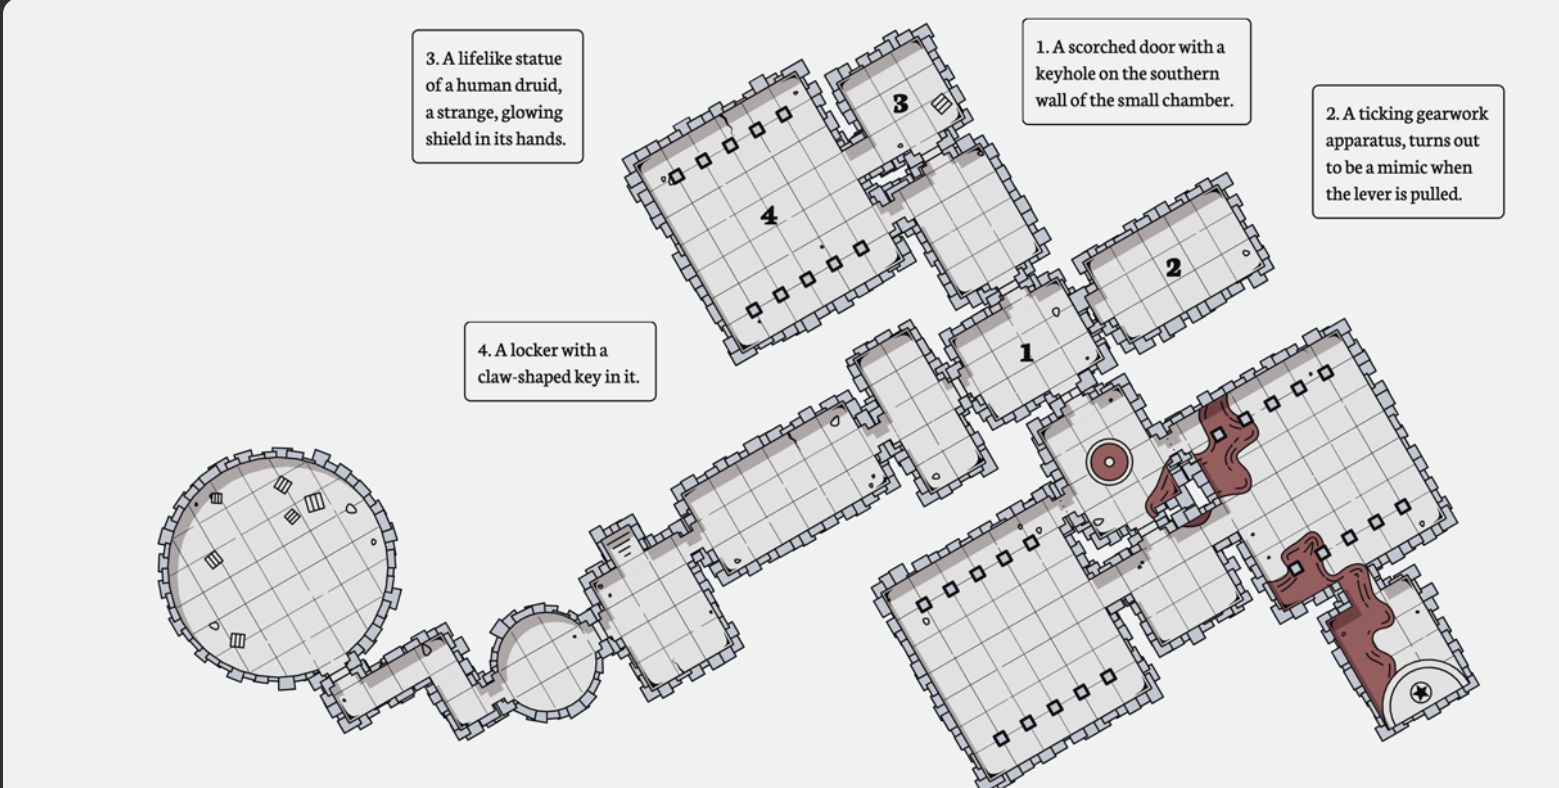
\includegraphics[width=0.5\linewidth]{watab.png}
    \caption{Watabou's Procgen Arcana}
    \label{fig:enter-label}
\end{figure}
I used the Procedural Dungeon Generation: A Drunkard's Walk in ClojureScript as inspiration for my early version of code. The blog post explores procedural dungeon generation using the "Drunkard's Walk" algorithm implemented in ClojureScript. The author discusses the algorithm's basics, where it starts from a point and randomly navigates the grid to create intricate maze-like structures. \cite{jrheard_dungeon_clojurescript}

\begin{figure}
    \centering
    
\includegraphics[width=0.5\linewidth]{mine.png}
    \caption{my output from inspiration from Procedural Dungeon Generation: A Drunkard's Walk in ClojureScript}
    \label{fig:enter-label}
\end{figure}


The post provides insights into the implementation details, including grid initialization, wall generation, and room placement. It also highlights how parameters like randomness and wall density affect the generated dungeons. The blog post offers a practical demonstration of the algorithm's capabilities, showcasing the creation of diverse and engaging dungeon layouts for game development or other applications. However, one of the project's shortcomings is it doesn't guarantee a map for adventure. Sometimes, it looks like a giant opening instead of a dungeon pattern.
Then I found this webpage. It simplifies the drunkard walk algorithm into four steps.:
\begin{enumerate}
    \item Pick a random point on a filled grid and mark it empty.
    \item Choose a random cardinal direction (N, E, S, W).
    \item Move in that direction, and mark it empty unless it already was.
    \item Repeat steps 2-3 until you have emptied as many grids as desired.\cite{pcgwiki_drunkardwalk}
\end{enumerate}

It is easy to follow, so I created my algorithm based on this blog.


\subsection{Methods}


The method employed for generating dungeon maps and boss room maps emphasizes the strategic application of logical constraints, creating unique and immersive gaming experiences. These algorithms stand out because they focus on diversifying room shapes, establishing interconnected layouts, and strategically placing rooms according to their designated types.

A key feature of the Random Dungeon Map Generator's approach is its utilization of various room shapes, including rectangles and circles of different sizes. This diversity enhances visual aesthetics and enriches gameplay by introducing rooms of varying sizes and functions. Meticulous care is taken to prevent room overlap or collision, preserving the overall integrity of the dungeon layout.

\begin{figure}
    \centering
    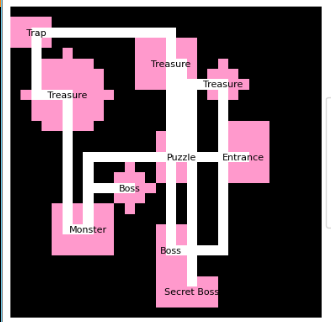
\includegraphics[width=0.5\linewidth]{mymap.png}
    \caption{Random Dungeon Map generator }
    \label{fig:enter-label}
\end{figure}

\begin{figure}
    \centering
    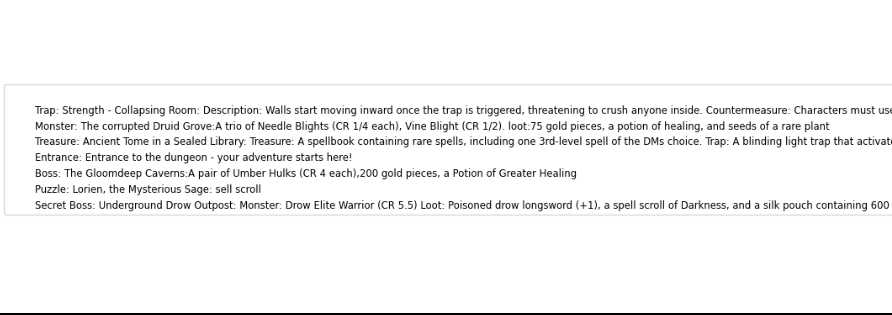
\includegraphics[width=0.5\linewidth]{desc.png}
    \caption{these are the descriptions for my map}
    \label{these are the descriptions for my map}
\end{figure}

The algorithm excels in logically connecting rooms by determining central points and calculating the shortest paths between them. This results in a network of passages seamlessly fitting into the dungeon's context, offering opportunities for exploration and encounters that feel organically integrated.

Another noteworthy feature is the algorithm's dynamic room captioning system. Each room can be assigned a label or caption, adding narrative depth to the dungeon. These captions are intelligently generated based on room type and default labels, enhancing the storytelling experience. For instance, the treasure room is consistently placed adjacent to the "boss" room, while weaker monsters are strategically positioned near puzzle rooms. This enriches player immersion by providing clues, challenges, or rewards aligned with their exploration.

In contrast to traditional "Drunkard's Walk" algorithms, which rely on random movements, this method adopts a more deliberate and controlled approach. It combines randomness in room generation with the logic of connectivity and narrative context, resulting in meticulously crafted dungeons that feel purposeful and engaging.

Comparing this approach to Watabou's one-page dungeon generator reveals distinctions. Watabou's tool creates one-page dungeons with varying themes butlacks detailed descriptions for monsters, loot, and additional elements, potentially limiting the Dungeons and Dragons (DnD) gaming experience for Dungeon Masters (DMs) and players.

To address these limitations, the algorithm is inspired by "Procedural Dungeon Generation: A Drunkard's Walk in ClojureScript." While this source introduced \cite{jrheard_dungeon_clojurescript}randomization, it occasionally led to caverns or openings lacking depth or purpose and did not offer means to incorporate objectives or encounters for players.

Hence, the algorithm takes a different approach, focusing on logical constraints for constructing dungeon layouts aligned with design and gameplay objectives. Although a decision tree could serve as an alternative, its complexity exceeds the current scope, making logical constraints a more suitable choice.

The Random Boss Room Generator implements a method for generating Dungeons and Dragons (DnD) boss room layouts using logical constraints and randomization. The algorithm begins by defining specific room types, each with a maximum allowable count, such as "Throne Room," "Entrance," "Bathroom," "Sleeping Area," "Torture Room," "Guard Room," "Treasure Room," and "Kitchen." These room types play vital roles in shaping the dungeon's layout and gameplay.
\begin{figure}
    \centering
    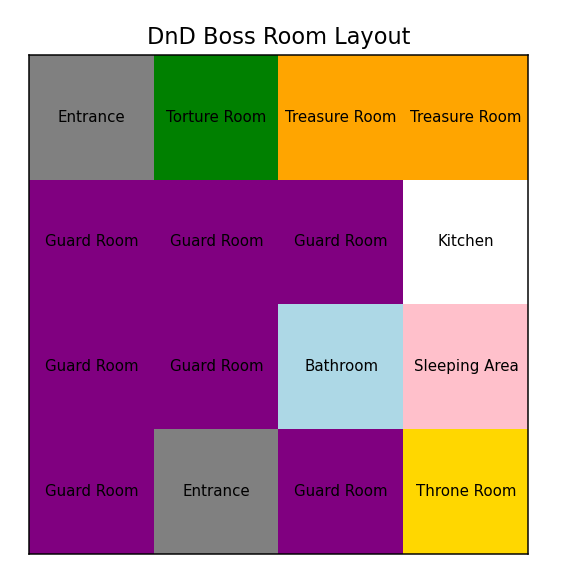
\includegraphics[width=0.5\linewidth]{bossmap.png}
    \caption{bossroom layout}
    \label{fig:enter-label}
\end{figure}
The algorithm starts by strategically placing the "Throne Room" farthest from the "Entrance," creating a spatial hierarchy that adds depth and anticipation to the dungeon exploration. It ensures that the "Entrance" is positioned at least three spaces away from the "Throne Room," maintaining a sense of distance and challenge for players. This initial placement sets the stage for the overall layout.

Additionally, the algorithm places certain rooms in proximity to others based on narrative logic. For example, it positions the "Sleeping Area" near the "Throne Room" and the "Kitchen" adjacent to the "Sleeping Area," creating a layout reminiscent of architectural design principles. This not only enhances the immersion of players but also introduces strategic complexity to the gameplay.

One significant feature is the placement of the "Guard Room," which can be near either the "Entrance" or the "Throne Room." This constraint aligns with narrative logic, suggesting that crucial areas in the dungeon are typically protected by guards. This strategic placement enhances both player immersion and the tactical depth of the gameplay, adding an element of challenge and realism.

The algorithm is designed to ensure that each room type adheres to its maximum allowable count while still producing a logically connected and engaging dungeon layout. It relies on a set of rules and checks to validate the placement of rooms, considering factors such as room type, proximity to other rooms, and constraints specific to certain room types.

In conclusion, the algorithm presents an approach to generating random boss room and  Dungeon map layouts that prioritize both logical spatial arrangements and storytelling immersion. By strategically placing rooms and adhering to predefined constraints, it produces well-designed and engaging dungeon layouts that enhance the overall gaming experience.

\section{Evaluation Metrics}

These are the evaluation metrics I created on the first day I designed the project.I think these are fitting for the project.

\begin{enumerate}
    \item \textbf{Good Storyline (Who What Why):}
    
    \textit{Importance:} A good storyline is crucial for engaging players in the game world. It provides context, purpose, and motivation for their actions. A well-crafted narrative can make the gameplay more immersive and enjoyable.\cite{reddit_dnd_campaign_fun}
    
    \item \textbf{Good Adversary (Motivation, Theme, Difficulty, Variation):}
    
    \textit{Importance:} The adversary or antagonist in a game adds challenge and conflict, making the gameplay interesting. Their motivation and theme contribute to the depth of the story. The difficulty and variation ensure that encounters with the adversary remain engaging and not repetitive.\cite{reddit_dnd_campaign_fun}
    
    \item \textbf{Good NPC (Background, Personality, Function):}
    
    \textit{Importance:} Non-player characters (NPCs) play a significant role in shaping the game world. Their backgrounds and personalities add richness to the narrative. Their functions can range from providing information to offering quests or trading, enhancing the player's experience.\cite{reddit_dnd_campaign_fun}
    
    \item \textbf{Good Resolution (Rewarding or not, Meaning):}
    
    \textit{Importance:} The resolution of the hero's journey is what players work toward. A rewarding resolution provides a sense of accomplishment and satisfaction, motivating players to continue or replay the game. The meaning or impact of the resolution can leave a lasting impression on players.\cite{reddit_dmacademy_oneshot}
    
    \item \textbf{Well-Constructed (What will the map look like, Theme, Difficulty):}
    
    \textit{Importance:} A well-constructed map is essential for navigation and exploration within the game. The map's theme sets the tone and atmosphere, enhancing immersion. Difficulty ensures that players are appropriately challenged, maintaining their interest.\cite{reddit_dmacademy_oneshot}
\end{enumerate}

A rewarding resolution provides a sense of achievement and closure, motivating players to complete the game and potentially play it again.
The importance of these metrics is justified in the context of game design literature, where a compelling narrative, challenging gameplay, and immersive world-building are often considered essential elements for successful games. These metrics help ensure that your algorithm generates game scenarios that are enjoyable, engaging, and memorable for players.



\section{Evaluation Results and Discussion}

Prior to conducting playtesting, I conducted interviews with five Dungeon Masters (DMs) on Discord channels, namely "DND Behind" and "Discord and Dragons." These interviews served as valuable sources of feedback and insights into the design and construction of the generated dungeon maps.

During the interviews, the DMs initially criticized the lack of content within the maps, particularly noting issues with the roads connecting each room. This feedback prompted a crucial refinement in the design process. I addressed these concerns by adding detailed descriptions to each room and revising the logic governing the connections between rooms. The revised approach aimed to enhance both the visual and narrative aspects of the maps, ensuring that players could better immerse themselves in the gaming experience.

Following these adjustments, I sought the opinions of the interviewed DMs on the overall construction of the maps. To my satisfaction, all of them affirmed that the maps were well-constructed. This validation encouraged me to proceed with playtesting to gain further insights into the maps' performance and gameplay experience.

The playtesting phase involved a group of student DMs and players who actively engaged with the maps. Despite only exploring a fraction of the entire map, the players invested an hour in navigating three rooms. Their engagement was a testament to the immersive nature of the maps and their alignment with the storytelling aspect of Dungeons and Dragons (DnD). Remarkably, some players remarked that the gameplay experience felt akin to a "real thing," highlighting the success of the immersion factor.

Subsequently, the DMs provided additional feedback based on their observations during the playtesting session. Their input emphasized the need for more logical room arrangements. They suggested that powerful monsters should not be placed immediately adjacent to the "boss" room, and puzzles should lead to rewards, enhancing the gameplay's strategic depth. Furthermore, they recommended adding more room descriptions to enrich the narrative aspect further.

In the players' assessment, the maps delivered a good storyline, and they appreciated how the narrative progressed as they played through the rooms. The online DMs also commended the overall structure of the maps. However, it is noteworthy that the student DMs expressed some dissatisfaction with the arrangement of the maps, desiring a more consistent placement of rooms labeled as "Treasure room" or "Boss room" in dead-end areas. Despite the limited exploration of rooms, the players encountered four distinct room types: "NPC room," "Trap room," "weak monster," and "strong monster." Their satisfaction with the variety and challenge posed by these rooms reflected positively on the map's design.

Regarding NPCs (Non-Player Characters), the players interacted with one NPC during the session, and their feedback indicated that the encounter was highly beneficial and engaging. However, the DMs raised concerns about NPCs' impact on in-game economy balance. The student DMs also recognized the flexibility of the map generator, noting that it could be adapted to suit different levels of gameplay, showcasing its versatility.

Despite these positive aspects, there are certain limitations to the current code. Notably, the placement of elements in dead-end areas is random, which can lead to a lack of consistency in their distribution. Additionally, the code's grouping of certain labels lacks a clear ordering mechanism. Addressing these issues would require a fundamental shift to a decision tree-based algorithm, which is not feasible at this stage of development. Furthermore, the hardcoded descriptions are not modular, making it challenging to adjust monster levels or loot automatically based on player preferences. The excessive length of descriptions has also been identified as an area for improvement. The student DMs suggested a feature that would provide full monster descriptions in a dropdown sheet or text file, enhancing user convenience.

Moving on to the Boss Room Map Generator, it introduces a set of constraints to create layouts that adhere to logical spatial arrangements and enhance storytelling immersion. However, the presentation of the generated layouts remains somewhat underwhelming, with the output being a 5x5 image resembling an apartment layout. While this design choice aligns with the concept, creating more intricate layouts would require graphic design software beyond Python's capabilities, presenting a knowledge limitation.

Furthermore, due to variations in room appearance rates, white space may be present in the generated maps. This issue has been mitigated by replacing such spaces with "guard rooms." While this solution maintains the overall structure, it highlights the need for further refinement in the layout generation process, particularly regarding guard room placement.

In conclusion, the interviews and playtesting sessions provided valuable insights into the strengths and limitations of the generated maps. The feedback received has been instrumental in refining the map generation algorithm to enhance content, logic, and descriptions. While certain challenges and limitations persist, the maps have demonstrated their potential to deliver engaging storytelling and gameplay experiences in the world of Dungeons and Dragons..

\section{Ethical Considerations}


Ethical considerations are of paramount importance in the development of procedural dungeon and boss room generators for tabletop role-playing games (TTRPGs). This project involves creating algorithms and systems that directly impact the gaming experience of players and Dungeon Masters (DMs). As such, it is crucial to address ethical concerns related to fairness, inclusivity, player agency, content appropriateness, and intellectual property. This document outlines the ethical considerations undertaken throughout the project's development.

1. Fairness and Inclusivity:
   - Fair Randomization: Ensuring that randomization algorithms do not result in excessively biased or unfair outcomes in gameplay, such as favoring certain players or punishing others unfairly.
   - Accessibility: Making sure that generated content is accessible to all players, including those with disabilities, by providing alternative formats, descriptions, and usability features.
   - Inclusivity: Avoiding content that promotes discrimination, stereotypes, or offensive themes and promoting inclusivity in character creation and storytelling.

2. Player Agency:
   - Transparency: Providing players and DMs with insights into how the procedural generation works to maintain the element of player agency and reduce feelings of helplessness.
   - Customization: Offering options for players and DMs to adjust algorithms, room placements, or other parameters to tailor the gaming experience to their preferences.
   - Balancing: Ensuring that generated challenges are appropriately balanced, allowing for meaningful choices and decision-making in gameplay.\cite{quinn2022ethics_rpg}

3. Content Appropriateness:
   - Age Appropriateness: Consider the age group of the players and ensure that generated content is suitable for the intended audience by avoiding explicit or mature themes.
   - Trigger Warnings: Providing warnings or opt-out options for content that may trigger emotional distress or discomfort in players.
   - Cultural Sensitivity: Avoiding content that may be culturally insensitive or appropriative and respecting cultural contexts in storytelling\cite{bourke2017morality_ethics_rpg}.

4. Intellectual Property:
   - Ownership: Respecting copyright and intellectual property rights when using third-party assets, ensuring proper attribution, and seeking necessary permissions.
   - Originality: Striving for originality in generated content and avoiding direct copying or replication of copyrighted materials.

5. Data Privacy:
   - Data Protection: Safeguarding any user data collected during gameplay, such as preferences or customizations, and ensuring compliance with data protection regulations.

6. Accountability:
   - Bug and Bias Detection: Implementing mechanisms to detect and address any biases or bugs that may impact gameplay, and taking prompt corrective actions.
   - Feedback Channels: Providing clear channels for users to report concerns or ethical issues related to generated content or gameplay.\cite{quinn2022ethics_rpg}

7. Continuous Improvement:
   - Iteration and Adaptation: Continuously assessing and improving the procedural generation algorithms based on user feedback and evolving ethical standards.
   - Staying Informed: Keeping up-to-date with developments in ethics within the gaming industry and TTRPG community to ensure alignment with best practices.

Ethical considerations are an integral part of developing procedural dungeon and boss room generators for TTRPGs. By prioritizing fairness, inclusivity, player agency, content appropriateness, respect for intellectual property, data privacy, accountability, and continuous improvement, developers can create experiences that are not only engaging and entertaining but also respectful of players' diverse backgrounds and preferences. Ethical choices contribute to the responsible and sustainable growth of this creative and dynamic field, ensuring that TTRPGs remain enjoyable and inclusive for all participants.

In addition to the foundational ethical considerations outlined above, it is essential to emphasize the iterative nature of ethical development in random dungeons and boss room generators. As the landscape of tabletop role-playing games evolves, so too should the ethical framework that guides their creation. This necessitates an ongoing commitment to staying informed about emerging ethical standards and community feedback.

Furthermore, fostering a culture of inclusivity and ethical responsibility within the gaming community is paramount. Encouraging players, DMs, and developers to engage in discussions about ethical considerations actively can lead to a more collaborative and accountable approach to game design.

Ultimately, by integrating ethical principles into the heart of procedural generation, we can ensure that tabletop role-playing games continue to be a source of enjoyment and inspiration for a diverse and growing community of players and creators.
\section{Conclusion}

In conclusion, the project of developing procedural dungeon and boss room generators for tabletop role-playing games (TTRPGs) has yielded promising results, addressing several critical aspects of game design and enhancing the overall player experience. We have focused on creating immersive, balanced, and ethical gaming environments throughout the project. As we reflect on the achievements and challenges encountered during this endeavor, it is clear that procedural generation has the potential to impact TTRPGs significantly and positively.

Key Achievements:
1. **Enhanced Gameplay**: The procedural dungeon generator has successfully created diverse and strategically structured dungeon layouts, offering players a more engaging and challenging experience. Including dynamic room, captions has added depth to storytelling, while the boss room generator has improved narrative coherence and tactical gameplay.

2. **Fairness and Inclusivity**: Ethical considerations have been central to my project, ensuring that generated content is fair, inclusive, and appropriate for diverse audiences. This approach promotes a welcoming and respectful gaming environment.

3. **Player Agency**: By allowing players and Dungeon Masters (DMs) to customize algorithms and adjust parameters, I have empowered them to tailor their TTRPG adventures to their preferences. Transparency in procedural generation further enhances player agency, fostering a sense of control and immersion.

4. **Content Appropriateness**: The project has prioritized age-appropriate content, trigger warnings, and cultural sensitivity, making TTRPGs accessible and enjoyable for many players. This approach helps prevent potentially uncomfortable or distressing experiences. All the players and the DMs are comfortable with the content I created.

5. **Ethical Considerations**: I have proactively addressed issues related to intellectual property, data privacy, and accountability, ensuring that the project aligns with ethical standards and legal requirements to my player and DMs.
\section{Future Work}
While the project has achieved several milestones, there is ample room for further development and improvement in the field of procedural dungeon and boss room generation for TTRPGs:

1. **Advanced Algorithms**: Future work can explore more sophisticated algorithms to create even more complex and dynamic dungeon layouts. Incorporating decision trees, machine learning, or neural networks may enable generators to adapt to player preferences and behaviors during gameplay.

2. **Multiplayer Integration**: Integrating multiplayer capabilities, allowing multiple players or DMs to collaboratively or competitively create and explore procedurally generated dungeons, can enhance the social aspect of TTRPGs.

3. **Enhanced Graphics and Visualization**: Improving the graphical representation of generated dungeons, potentially through the integration of graphic design software or 3D modeling, can provide a more immersive visual experience.

4. **Natural Language Processing**: Incorporating natural language processing to generate detailed descriptions of rooms, NPCs, and encounters could further enrich storytelling and reduce the need for manually entering room descriptions.

5. **Player Feedback Mechanisms**: Developing systems for players to provide feedback on generated content and gameplay experiences can help fine-tune algorithms and identify areas for improvement.

6. **Expansion into Other TTRPG Systems**: Adapting the procedural generation tools to work seamlessly with various TTRPG systems beyond Dungeons & Dragons, such as Pathfinder or Call of Cthulhu, would broaden the project's applicability.

7. **Educational Applications**: Exploring how procedural generation can be used for educational purposes, such as teaching game design or history through TTRPG scenarios, can open up new avenues for the project.

8. **Dynamic Difficulty Scaling**: Implementing mechanisms that dynamically adjust dungeon difficulty based on player skill, character level, or party composition can create more tailored and challenging experiences.

9. **Storyline Integration**: Integrating procedural generation into overarching campaign storylines, allowing generated content to align more closely with the narrative, can enhance immersion and coherence.

10. **Cross-Platform Compatibility**: Ensuring that the procedural generation tools are compatible with various platforms, including virtual tabletop systems and mobile devices, can broaden their accessibility.

In summary, the project has made significant strides in developing procedural dungeon and boss room generators for TTRPGs, emphasizing fairness, inclusivity, and ethical considerations. The potential for growth and innovation in this field is substantial, offering exciting opportunities to enhance TTRPG experiences for players and DMs. By continuing to refine algorithms, expand capabilities, and embrace emerging technologies, we can look forward to a future where procedurally generated content plays an even more significant role in tabletop role-playing games.


\section{Timeline}

I commenced this project in the second week of the semester, and as I prepared for my initial presentation, I was uncertain about the path to success. In early October, a significant breakthrough occurred when I developed a program based on the Drunkard's Walk algorithm. However, I found this approach to be overly simplistic. Subsequently, in late October, I completed the prototype for my current project. Following a month of coding and refining, I conducted playtesting at the end of November. Additionally, I successfully created a boss room generator, which involved more intricate constraints than the dungeon map generator. Currently, I am in the process of composing this essay

\section{Replication Instructions}
\section{Prerequisites}

Make sure you have the following prerequisites installed on your system:

\begin{itemize}
    \item Python (3.x recommended)
    \item Matplotlib
    \item NumPy
\end{itemize}

You can install Matplotlib and NumPy using pip:

\begin{lstlisting}[language=bash]
pip install matplotlib numpy
\end{lstlisting}
\section{Tutoiral for Dungeonmap.py}
\subsection{Step 1: Clone the Repository (If Applicable)}

If your code is part of a Git repository, clone it to your local machine:

\begin{lstlisting}[language=bash]
git clone <https://github.com/VictorZhudd/senior-comp2.git>
cd <repository_directory>
\end{lstlisting}

\subsection{Step 2: Open the Python Script and make sure bossroom.py is in the folder}

Open the Python script where you've pasted the provided code. Let's call it \texttt{dungeonmap.py}. Since the code will create not only a dungeon map but also a boss room map, the user must find a function called generate\_dnd\_boss\_room\_layout\_v8 in another script. In my package, you can find it in bossroom.py

\subsection{Step 3: Adjust Room Type Chances}

You can customize the chance of different room types appearing by modifying the \texttt{group\_params} list. Each element in this list represents a group of rooms with associated labels, shapes, and chances.

For example, if you want to increase the chance of "Treasure" rooms appearing, change the chance value (between 0.0 and 1.0) in the \texttt{group\_params} list. Here's how:

\begin{lstlisting}[language=Python]
group_params = [
    (['Treasure', 'Puzzle'], ['rectangle', 'rectangle'], [0.8, 1.0]),  # Increase chance for 'Treasure'
    (['Treasure', 'Strong Monsters'], ['rectangle', 'circle'], [0.2, 0.6]),
    # Add or modify other room groups as needed
]
\end{lstlisting}

\subsection{Step 4: Define Custom Colors}

To define custom colors for room visualization, you can modify the \texttt{colors} array and the \texttt{cmap} colormap. The \texttt{colors} array represents the RGB colors for different room types, and the \texttt{cmap} is the colormap that uses these colors.

Here's how to define custom colors:

\begin{lstlisting}[language=Python]
colors = np.array([
    [0, 0, 0],     # Black for walls (-1)
    [0.8, 0.8, 0.2], # Custom color for 'Treasure' rooms (0)
    [1, 1, 1],     # White for paths (1)
])
cmap = ListedColormap(colors)
\end{lstlisting}

You can adjust the RGB values to specify different colors for each room type.

\subsection{Step 5: Customize Room Descriptions}

Customize room descriptions by modifying the \texttt{room\_descriptions} dictionary. Add or modify descriptions for each room type as needed.

Here's an example of custom room descriptions:

\begin{lstlisting}[language=Python]
room_descriptions = {
    'Treasure': [
        'A glittering treasure chest awaits! It contains a valuable gem.',
        'You found a hidden stash of gold coins and jewelry!',
    ],
    'NPC': [
        'You encounter a friendly merchant who offers to trade with you.',
        'A mysterious traveler shares valuable information about the dungeon.',
    ],
    # Add or modify descriptions for other room types
}
\end{lstlisting}

\subsection{Step 6: Specify Room Dimensions and Map Size}

You can specify the dimensions of rooms and the size of the grid by modifying relevant parameters in the code. For example, to change the minimum and maximum room dimensions, modify the following lines:

\begin{lstlisting}[language=Python]
room_width = random.randint(3, 6)  # Change the range as needed
room_height = random.randint(3, 6)  # Change the range as needed
\end{lstlisting}

Also, define the dimensions of the grid by changing the \texttt{width} and \texttt{height} variables:

\begin{lstlisting}[language=Python]
width, height = 30, 30  # Change to your desired map size
\end{lstlisting}

\section{Step 7: Run the Script}

Save your changes and run the script:

\begin{lstlisting}[language=bash]
python dungeonmap.py
\end{lstlisting}
and it should come out likes this:
\begin{figure}
    \centering
    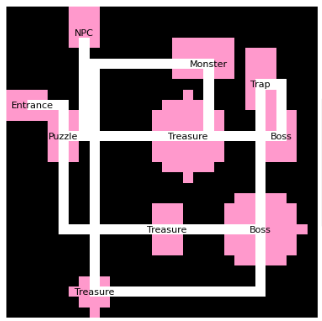
\includegraphics[width=0.5\linewidth]{example1.png}
    \caption{the map part of you result should look like this}
    \label{fig:enter-label}
\end{figure}

\begin{figure}
    \centering
    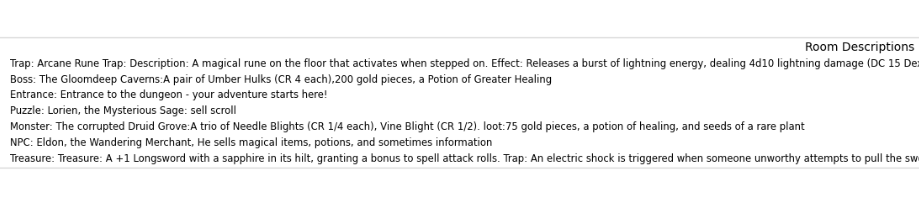
\includegraphics[width=0.5\linewidth]{decs.png}
    \caption{the map should come with these descriptions}
    \label{fig:enter-label}
\end{figure}
it will also trigger bossroom.py and create a boss room map
\section{Tutorial for bossroom.py}
This tutorial provides an interactive guide to enhancing your DnD Boss Room Layout script. It will walk you through the features of the script and demonstrate how to effectively use and modify them to create compelling dungeon designs. This script connects to the dungeonmap.py. It needs both scripts to work.

\subsection{Exploring the Script's Features}
\subsubsection{Creating a Diverse Array of Rooms}
The heart of the script lies in its ability to create various room types. This diversity is managed through a dictionary named \texttt{room\_types}. Here's how to use it:

\begin{itemize}
    \item \textbf{Adding a New Room Type:} To introduce a new room, such as a 'Mystical Study', simply add it to the dictionary with a maximum count. For example:
    \begin{lstlisting}[language=Python]
    room_types["Mystical Study"] = 1
    \end{lstlisting}

    \item \textbf{Changing Room Names:} Modify the keys in the \texttt{room\_types} dictionary to rename rooms.
\end{itemize}

\subsubsection{Customizing the Dungeon Layout}
The layout is represented by a grid, initialized based on a specified size. This grid forms the blueprint of your dungeon. You can easily change the size of the grid to make your dungeon larger or smaller, thus altering the complexity and exploration opportunities.

\subsubsection{Strategically Placing Key Rooms}
The script includes logic for strategically placing important rooms like the Throne Room and the Entrance. You can modify this logic to change the layout dynamics, creating new challenges and narratives.

\subsubsection{Ensuring Logical Room Placement}
The function \texttt{is\_valid\_placement} checks if the placement of a room adheres to the dungeon theme and logic. Modifying this function allows you to set new rules for where specific rooms can be placed.

\subsubsection{Filling the Grid with Adventure}
After setting the key rooms, the script fills in the remaining spaces. This step is crucial for ensuring that every part of your dungeon is engaging. You can modify the filling logic to control the distribution of room types, balancing between challenge and exploration.

the default result should look like this
\begin{figure}
    \centering
    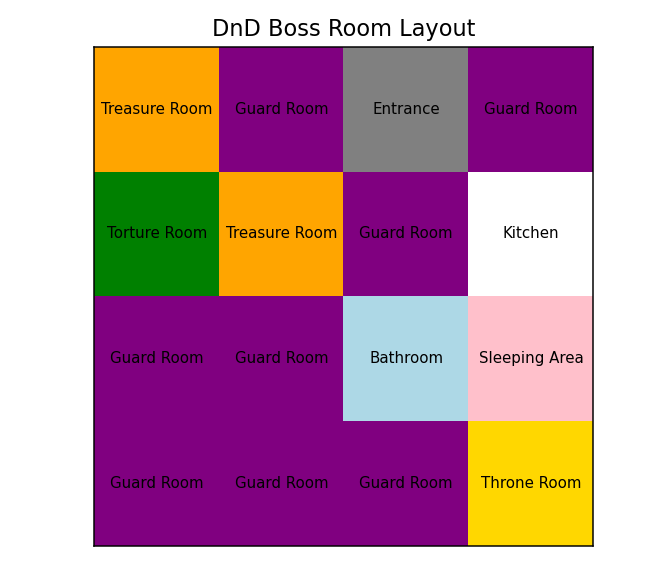
\includegraphics[width=0.5\linewidth]{bossroom.png}
    \caption{default bossroom.py result should look like this}
    \label{fig:enter-label}
\end{figure}
\subsection{Bringing Your Dungeon to Life: A Step-by-Step Example}
Let's go through an example of adding a 'Library' room to your dungeon:

\begin{lstlisting}[language=Python]
# Step 1: Add the Library to room_types
room_types["Library"] = 1

# Step 2: Assign a color to the Library in room_colors
room_colors["Library"] = "saddlebrown"

# Step 3: Modify is_valid_placement for the Library
# Add your custom logic here

# Step 4: Generate the dungeon layout
dnd_room_layout = generate_dnd_boss_room_layout_v8(6)
\end{lstlisting}



\section{Code Architecture Overview}

This section provides a detailed overview of the code architecture for two Python scripts: `bossroom.py` and `dungeonmap.py`. These scripts are designed to generate a Dungeons and Dragons (DND) dungeon layout, including a specific boss room.

\subsection{bossroom.py Overview}
\subsubsection{Purpose}
The `bossroom.py` script is designed to generate a layout for a D\&D boss room. 

\subsubsection{Key Components}
\begin{itemize}
    \item Room Types and Counts: Defines various D\&D room types and their maximum counts.
    \item Grid Initialization and Room Placement: Initializes a grid and places rooms based on specific rules.
    \item Plot Function: A function to visualize the generated room layout.
\end{itemize}

\subsection{Code Structure and Logic}
The script is structured with a clear separation between layout generation and visualization, using a mix of deterministic and random room placements.

\subsection{dungeonmap.py Overview}
\subsection{Purpose}
The `dungeonmap.py` script generates a larger dungeon map that includes the boss room.

\subsubsection{Key Components}
\begin{itemize}
    \item Grid Initialization: Initializes a grid for the dungeon map.
    \item Room Generation Functions: Functions to create and place various room types.
    \item Map Visualization: Visualizes the dungeon map with labels and descriptions.
\end{itemize}

\subsubsection{Integration with bossroom.py}
The script integrates with `bossroom.py` to incorporate the boss room layout into the larger dungeon map.

\subsection{Combined Code Architecture}
The scripts exhibit modular design, with each handling specific aspects of map generation. This modular approach aids in the readability and maintainability of the code.

\subsection{Recommendations for Future Development}
\begin{itemize}
    \item Enhance documentation and comments for clarity.
    \item Maintain modularity for ease of extending or debugging.
    \item Implement robust error handling for inputs and grid operations.
\end{itemize}


\printbibliography

\end{document}
